\documentclass[border=4pt]{standalone}
\usepackage{tikz}
\usepackage{pgfplots}
\pgfplotsset{compat=1.18}
\usetikzlibrary{plotmarks}

\definecolor{cNOOA}{RGB}{31,119,180}    % blue
\definecolor{cBASE}{RGB}{23,165,137}    % teal (unused; NOOA-base removed)
\definecolor{cOC}{RGB}{230,126,34}      % orange
\definecolor{cPI}{RGB}{155,89,182}      % purple

% marker size = reasoning effort
\newcommand{\szoff}{1.7}
\newcommand{\szhi}{3.2}
\newcommand{\szxhi}{4.8}
\newcommand{\sqoff}{1.7}
\newcommand{\sqhi}{3.2}

\tikzset{
  lead/.style={gray!55, line width=0.3pt},
  lab/.style={font=\scriptsize, inner sep=1pt},
}

\begin{document}
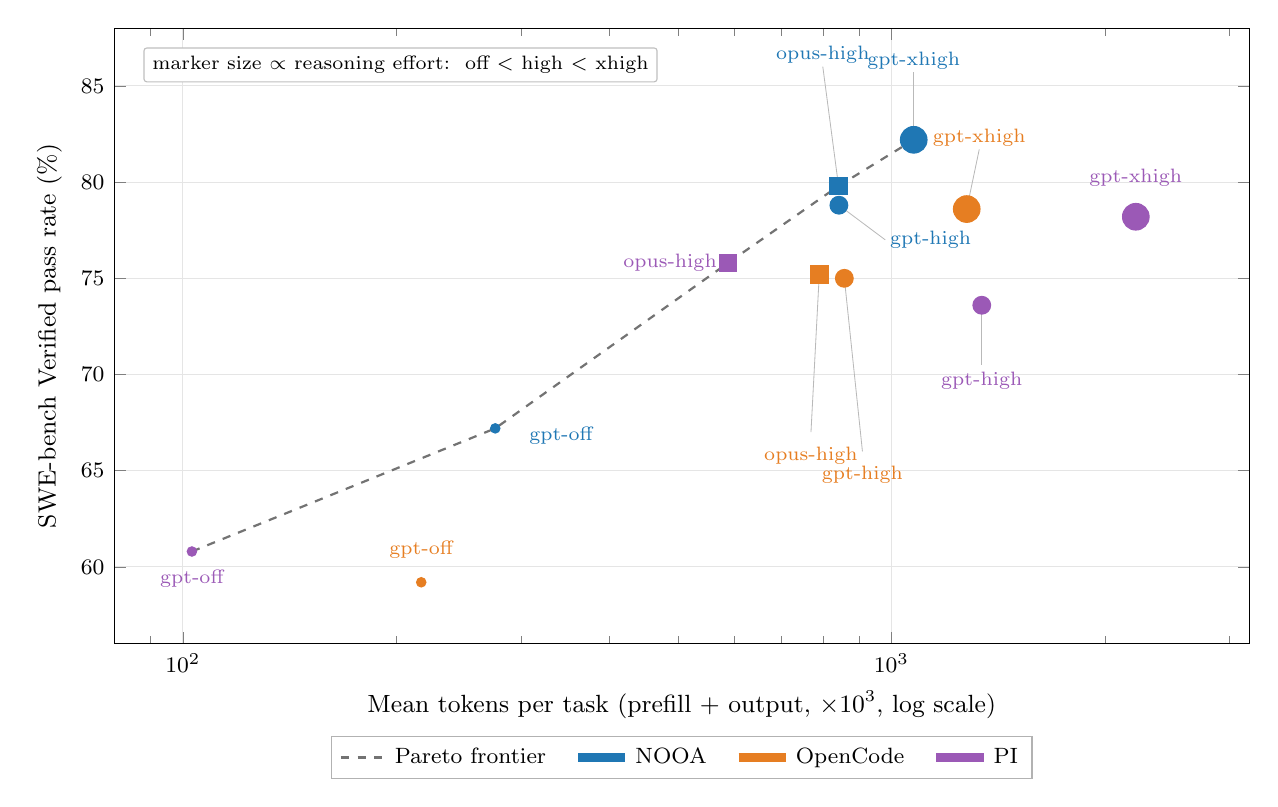
\begin{tikzpicture}
\begin{semilogxaxis}[
  width=16cm, height=9.4cm,
  xlabel={Mean tokens per task (prefill + output, $\times 10^3$, log scale)},
  ylabel={SWE-bench Verified pass rate (\%)},
  xmin=80, xmax=3200, ymin=56, ymax=88,
  grid=major, grid style={black!10},
  legend cell align=left,
  legend style={
    at={(0.5,-0.15)}, anchor=north, legend columns=4,
    font=\footnotesize, draw=black!30,
    /tikz/every even column/.append style={column sep=8pt},
  },
  tick label style={font=\footnotesize}, label style={font=\small},
]
% ===== effort-size key =====
\node[anchor=north west, font=\scriptsize, align=left, draw=black!25, fill=white,
      rounded corners=1pt, inner sep=3pt] at (axis cs:88,87)
  {marker size $\propto$ reasoning effort:\ \ off $<$ high $<$ xhigh};

% ===== Pareto frontier (gpt + opus, without NOOA-base) =====
\addplot[black!55, dashed, thick, mark=none] coordinates {
  (103,60.8) (276,67.2) (588,75.8) (842,79.8) (1075,82.2)};
\addlegendentry{Pareto frontier}

% ===== leader lines =====
\draw[lead] (axis cs:791,75.2) -- (axis cs:770,67);
\draw[lead] (axis cs:842,79.8) -- (axis cs:800,86);
\draw[lead] (axis cs:843,78.8) -- (axis cs:980,77);
\draw[lead] (axis cs:858,75.0) -- (axis cs:910,66);
\draw[lead] (axis cs:1075,82.2) -- (axis cs:1075,85.7);
\draw[lead] (axis cs:1277,78.6) -- (axis cs:1330,81.7);
\draw[lead] (axis cs:1341,73.6) -- (axis cs:1341,70.5);

% ===== markers: color=harness, shape=backend, size=effort =====
% NOOA (blue)
\addplot[forget plot,only marks,mark=*,      mark size=\szoff pt, cNOOA] coordinates {(276,67.2)};
\addplot[forget plot,only marks,mark=*,      mark size=\szhi pt,  cNOOA] coordinates {(843,78.8)};
\addplot[forget plot,only marks,mark=*,      mark size=\szxhi pt, cNOOA] coordinates {(1075,82.2)};
\addplot[forget plot,only marks,mark=square*,mark size=\sqhi pt,  cNOOA] coordinates {(842,79.8)};
% OpenCode (orange)
\addplot[forget plot,only marks,mark=*,      mark size=\szoff pt, cOC] coordinates {(217,59.2)};
\addplot[forget plot,only marks,mark=*,      mark size=\szhi pt,  cOC] coordinates {(858,75.0)};
\addplot[forget plot,only marks,mark=*,      mark size=\szxhi pt, cOC] coordinates {(1277,78.6)};
\addplot[forget plot,only marks,mark=square*,mark size=\sqhi pt,  cOC] coordinates {(791,75.2)};
% PI (purple)
\addplot[forget plot,only marks,mark=*,      mark size=\szoff pt, cPI] coordinates {(103,60.8)};
\addplot[forget plot,only marks,mark=*,      mark size=\szhi pt,  cPI] coordinates {(1341,73.6)};
\addplot[forget plot,only marks,mark=*,      mark size=\szxhi pt, cPI] coordinates {(2212,78.2)};
\addplot[forget plot,only marks,mark=square*,mark size=\sqhi pt,  cPI] coordinates {(588,75.8)};

% ===== legend: harness colors only =====
\addlegendimage{cNOOA, line width=3.2pt, mark=none}\addlegendentry{NOOA}
\addlegendimage{cOC,   line width=3.2pt, mark=none}\addlegendentry{OpenCode}
\addlegendimage{cPI,   line width=3.2pt, mark=none}\addlegendentry{PI}

% ===== labels (backend-effort), color = harness =====
% gpt-off (left)
\node[lab,cPI,  anchor=north] at (axis cs:103,60.0) {gpt-off};
\node[lab,cOC,  anchor=south] at (axis cs:217,60.3) {gpt-off};
\node[lab,cNOOA,anchor=west]  at (axis cs:305,66.8) {gpt-off};
% opus-high
\node[lab,cPI,  anchor=east]  at (axis cs:573,75.8) {opus-high};
\node[lab,cOC,  anchor=north] at (axis cs:770,66.4) {opus-high};
\node[lab,cNOOA,anchor=south] at (axis cs:800,86.0) {opus-high};
% gpt-high
\node[lab,cNOOA,anchor=west]  at (axis cs:985,77.0) {gpt-high};
\node[lab,cOC,  anchor=north] at (axis cs:910,65.4) {gpt-high};
\node[lab,cPI,  anchor=north] at (axis cs:1341,70.3) {gpt-high};
% gpt-xhigh
\node[lab,cNOOA,anchor=south] at (axis cs:1075,85.7) {gpt-xhigh};
\node[lab,cOC,  anchor=south] at (axis cs:1330,81.7) {gpt-xhigh};
\node[lab,cPI,  anchor=south] at (axis cs:2212,79.6) {gpt-xhigh};

\end{semilogxaxis}
\end{tikzpicture}
\end{document}
